\newpage
\newsection{CQRS}
Command Query Responsibility Segregation (CQRS) is an architectural pattern which separates the responsibility for modifying data (Command) from reading them (Query). The use of two different models for writing and reading operations, in scope of CQRS, allows instead to design and optimize each model for its responsibilities. In addition to this, the use of distinct models also allows the selection of the most appropriate technologies. As soon as the reading and writing models are separated, the infrastructure could easily scale to best fit the needs. It often happens that the number of writings in a system is much lower than the readings. Obviously the two models must be synchronized to ensure that the read information are consistent with the written ones.\\
The justification for CQRS is that in complex domains, a single model to handle both reads and writes gets too complicated, and we can simplify by separating the models.\\
The change that CQRS introduces is to split that conceptual model into separate models for update and display, which it refers to as Command and Query.\\
CQRS fits well with event-based programming models. It's common to see CQRS system split into separate services communicating with Event Collaboration. This allows these services to easily take advantage of Event Sourcing.


\subsection{Architecture overview}
\begin{figure} [H]
	\centering
	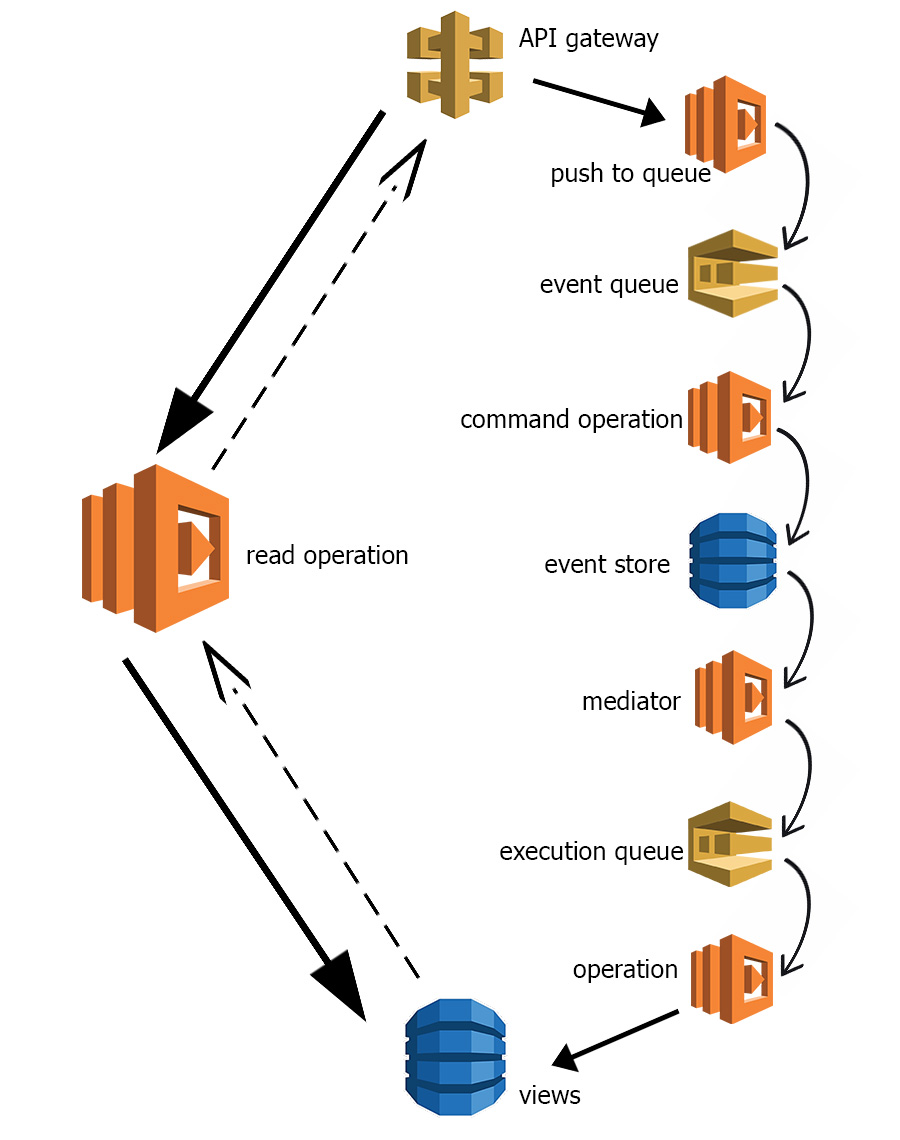
\includegraphics[scale=0.55]{../Img/architecture}
	\caption{Architecture overview}\label{}
\end{figure}
As you can see from the architecture overview, the application is separated into two models: write model(right side) and read model(left side). \\
The choice to apply the CQRS pattern due to separate the responsibilities of writing and reading, but also because read side events aren't stored into the event store table because they don't change the system's state but just retrieve information from it.


\subsection{Write model}
\begin{figure} [H]
	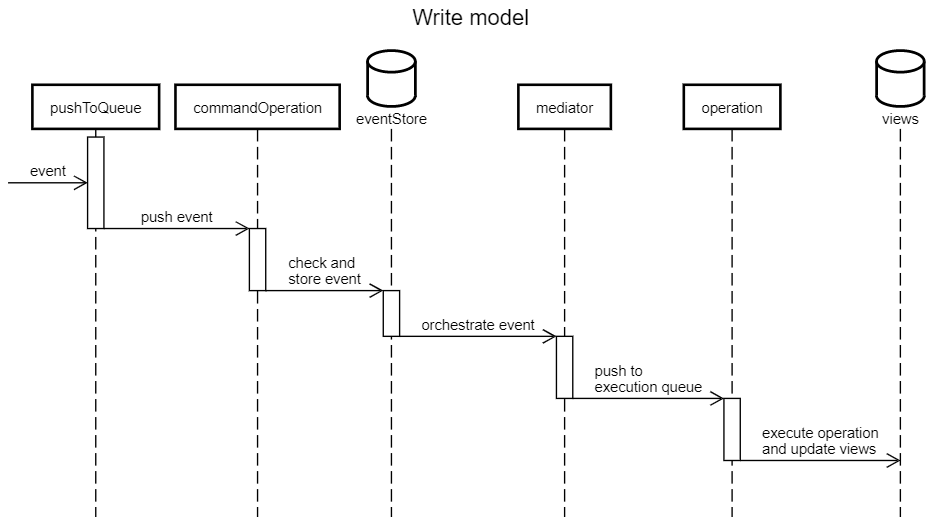
\includegraphics[scale=0.5]{../Img/write_model}
	\caption{Write model sequence diagram}\label{}
\end{figure}

\subsection{Read model}
\begin{figure} [H]
	\centering
	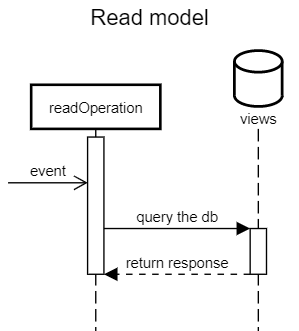
\includegraphics[scale=0.55]{../Img/read_model}
	\caption{Read model sequence diagram}\label{}
\end{figure}
